\documentclass[12pt]{article}

\usepackage{amsmath, mathtools, amssymb}
\usepackage[margin=0.5in]{geometry}
\usepackage[document]{ragged2e}
\usepackage{tikz}
\usepackage{undertilde}
\usepackage{graphicx}
\graphicspath{ {./images/} }

\makeatletter
\renewcommand*\env@matrix[1][*\c@MaxMatrixCols c]{%
  \hskip -\arraycolsep
  \let\@ifnextchar\new@ifnextchar
  \array{#1}}
\makeatother
\newcommand{\norm}[1]{\left\lVert#1\right\rVert}

\newcommand{\Lim}[1]{\raisebox{0.5ex}{\scalebox{0.8}{$\displaystyle \lim_{#1}\;$}}}

\newcommand{\vect}[1]{\boldsymbol{#1}}

\begin{document}
Vector Calculus Mast 20009 \hfill Felix McCuaig, 1159424 \\
Assignment 2 \hfill Tutorial Wed 5:15PM  

\section*{Question 1}
Let $D=\{ (x,y) \in \mathbb{R} \hspace{5px} | \hspace{5px} x^2+y^2\leq 1 \}$ and consider the function
$$
	f(x,y)=2x^2+y^2-y+3
$$
\textbf{(a)} Find and classify the local extrema of $f$ on the interior of the domain $D$.\\
\medskip
Let's use $\nabla f = 0$ to find extrema of $f$, then we can check if it's in $D$.\\
$$
\nabla f = (4x, 2y-1)
$$

When $\nabla f = 0$:
\begin{align*}
	4x &= 0 \rightarrow x = 0 \\
	2y-1 &=0 \rightarrow y = \frac{1}{2}\\
\end{align*}

To check that $\left(0, \frac{1}{2}\right)$ lies in $D$, we can compute $x^2+y^2$ and check that the result is $\leq  1$.
$$
	0^2+\frac{1}{2}^2=\frac{1}{4}, \hspace{20px} \frac{1}{4} \leq 1 
$$

Now, let's classify the extrema using the Hessian and partial derivatives.
\begin{align*}
	f_{xx} &= 4 \\
	f_{yy} &= 2 \\
	f_{xy} &= 0 \\
\end{align*}

$$
	H_f =
\begin{vmatrix}
f_{xx} & f_{xy} \\
f_{xy} & f_{yy} \\
\end{vmatrix}
=
\begin{vmatrix}
4 & 0 \\
0 & 2 \\
\end{vmatrix}
= 8
$$

Since $H_f > 0$ and $f_{xx} > 0$, the point $(0, \frac{1}{2})$ is a local min.\\
\medskip
\textbf{(b)} Use Lagrange multipliers to find the extrema of $f$ on the boundary of $D$.\\
\medskip
If we let $g(x,y)=x^2+y^2-1$, then we can find critical points on the boundary of $D$ using:
\begin{align*}
\nabla f &= \lambda \nabla g \\
\begin{bmatrix}
4x \\
2y - 1 \\
\end{bmatrix} &= \lambda 
\begin{bmatrix}
2x \\
2y \\
\end{bmatrix} \\
\end{align*}

This yields two equations:
\begin{align}
	4x = \lambda 2x \\
	2y-1 = \lambda 2y
\end{align}
From $(1)$, we get:
$$
x(4-2\lambda) = 0, \hspace{20px} x = 0 \text{ or } \lambda = 2
$$ 

For the case $x = 0$:
$$
0^2+y^2=1, \hspace{10px} y=\pm 1
$$

$$
\Rightarrow \left( 0, 1 \right), \left( 0, -1 \right)
$$
For the case $\lambda = 2$:
$$
2y-1 = 2 \times 2y \rightarrow -1 = 2y \hspace{10px} \therefore y= -\frac{1}{2}
$$
Then, as before, we can use:
$$
x^2+ \left( \frac{-1}{2} \right)^2=1 \rightarrow x^2 = \frac{3}{4} \hspace{20px} \therefore x = \pm \frac{\sqrt{3}}{2}
$$
$$
\Rightarrow \left( \frac{\sqrt{3}}{2}, \frac{-1}{2} \right), \left( \frac{-\sqrt{3}}{2}, \frac{-1}{2} \right)
$$

\medskip
\textbf{(c)} Use the results of the previous parts to determine the extrema of $f$ on the domain $D$.\\
\medskip

$$
f\left(0, \frac{1}{2}\right)=2(0)^2+\left( \frac{1}{2} \right)^2-\frac{1}{2}+3=\frac{1}{4}-\frac{2}{4}+\frac{12}{4}=\frac{11}{4}
$$

$$
f(0, 1)=2(0)^2+(1)^2-1+3=3
$$

$$
f(0, -1)=2(0)^2+(-1)^2+1+3=5
$$

$$
f\left( \frac{\sqrt{3}}{2}, \frac{-1}{2} \right)=2\left( \frac{\sqrt{3}}{ 2 } \right)^2+\left( -\frac{1}{2} \right)^2+\frac{1}{2}+3=2 \cdot \frac{3}{4} + \frac{1}{4} + \frac{1}{2} + 3 = 5 + \frac{1}{4}
$$

$$
f\left( \frac{-\sqrt{3}}{2}, \frac{-1}{2} \right)=2\left( -\frac{\sqrt{3}}{ 2 } \right)^2+\left( -\frac{1}{2} \right)^2+\frac{1}{2}+3=2 \cdot \frac{3}{4} + \frac{1}{4} + \frac{1}{2} + 3 = 5 + \frac{1}{4}
$$

Hence, $\left(1, \frac{1}{2} \right)$ is the global min of $f$ on $D$. $(0, 1)$ is a local min on the boundary of $D$, $(0, -1)$ is a local min on the boundary of $D$ and $\left( \frac{\sqrt{3}}{2}, \frac{-1}{2} \right)$ and $\left( \frac{-\sqrt{3}}{2}, \frac{-1}{2} \right)$ are local maximums on the boundary of $D$. See cool graphic:\\

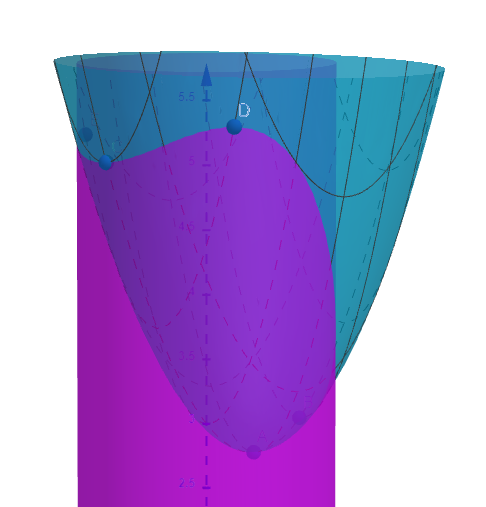
\includegraphics[width=10cm]{image1}

\section*{Question 2}
Compute the torsion of the curve
$$
\vect{\gamma}(t)=(at, \sin(bt), \cos(bt)), \hspace{20px} a,b > 0
$$

Let's first find the unit tangent vector for some $\vect{c}(t)$ which so happens to be $\vect{\gamma}(t)$:\\

$$
\vect{T}(t)=\frac{\frac{d\vect{c}}{dt}}{|\frac{d\vect{c}}{dt}|}=\frac{\frac{d\vect{\gamma}}{dt}}{|\frac{d\vect{\gamma}}{dt}|}
$$

$$
\frac{d\gamma}{dt}= (a, b \cos(bt), -b \sin(bt))
$$

$$
\left|\frac{d\gamma}{dt}\right|= \sqrt{a^2+b^2 \cos(bt)+b^2 \sin(bt)}=\sqrt{a^2+b^2}
$$

$$
\vect{T}(t)=\frac{(a, b \cos(bt), -b \sin(bt))}{\sqrt{a^2+b^2}}
$$
Now, let's find a unit normal vector $\vect{N}(t)$:
$$
\vect{N}(t)=\frac{\frac{d \vect{T}}{dt}}{\left| \frac{d \vect{T}}{dt}\right|}
$$
$$
\frac{d \vect{T}}{dt}=\frac{1}{\sqrt{a^2+b^2}}\left(0, -b^2\sin(bt), b^2\cos(bt)\right)
$$
$$
\left|\frac{d \vect{T}}{dt} \right|=\frac{b^2}{\sqrt{a^2+b^2}}
$$

$$
\vect{N}(t)=\frac{1}{\sqrt{a^2+b^2}}\left(0, -\sin(bt), \cos(bt)\right)
$$

$$
\vect{B}(t)=\vect{T}\times\vect{N}=
\begin{vmatrix}
	\vect{i} & \vect{j} & \vect{k} \\
	\frac{a}{\sqrt{a^2+b^2}} & \frac{b \cos(bt)}{\sqrt{a^2+b^2}} & \frac{-b \sin(bt)}{\sqrt{a^2+b^2}} \\
	0 & \frac{-\sin(bt)}{\sqrt{a^2+b^2}} & \frac{\cos(bt)}{\sqrt{a^2+b^2}} \\
\end{vmatrix}
=
\begin{bmatrix}
	\frac{b\cos^2(bt)}{a^2+b^2} - \frac{b\sin^2(bt)}{a^2+b^2} \\
	- \frac{a\cos(bt)}{a^2+b^2} \\
	- \frac{a\sin(bt)}{a^2+b^2}
\end{bmatrix}
$$

$$
\vect{B}(t)=
\left( 
	\frac{b\cos^2(bt)}{a^2+b^2} - \frac{b\sin^2(bt)}{a^2+b^2},
	- \frac{a\cos(bt)}{a^2+b^2},
	- \frac{a\sin(bt)}{a^2+b^2} 
\right)
$$
The torsion $\tau$ can be calculated as:
$$
\tau = \frac{\frac{d \vect{B}}{dt}}{\left| \frac{d\vect{c}}{dt} \right|}\cdot \vect{N}
$$

$$
	\frac{d \vect{B}}{dt} = \left( 0, \frac{ab\sin(bt)}{a^2+b^2}, -\frac{ab\cos(bt)}{a^2+b^2}\right)
$$
Remember that:
$$
	\left|\frac{d\gamma}{dt}\right|= \sqrt{a^2+b^2 \cos(bt)+b^2 \sin(bt)}=\sqrt{a^2+b^2}
$$
So:
$$
\tau = \frac{\left( 0, \frac{ab\sin(bt)}{a^2+b^2}, -\frac{ab\cos(bt)}{a^2+b^2}\right)}{\sqrt{a^2+b^2}}\cdot \frac{1}{\sqrt{a^2+b^2}}\left(0, -\sin(bt), \cos(bt)\right)
$$

$$
\tau = \frac{\left( 0, \frac{ab\sin(bt)}{a^2+b^2}, -\frac{ab\cos(bt)}{a^2+b^2}\right)}{\sqrt{a^2+b^2}}\cdot \frac{1}{\sqrt{a^2+b^2}}\left(0, -\sin(bt), \cos(bt)\right)
$$

$$
\tau = \frac{-a\cdot b}{(a^2+b^2)^2}
$$
\section*{Question 3}
Let $\vect{r}=x\vect{i}+y\vect{j}+z\vect{k}$ and $r=||\vect{r}||$. Let $f:[0,\infty )\rightarrow \mathbb{R} $ be a differentiable scalar function. Prove that\\
$$
\nabla \cdot (f(r)\vect{r})=r\frac{df}{dr}+3f(r)
$$
Let's start with:
\begin{align*}
&=\nabla \cdot (f(r)\vect{r})\\
&=\begin{bmatrix}
\frac{\partial}{\partial x} \\
\frac{\partial}{\partial y} \\
\frac{\partial}{\partial z}
\end{bmatrix}
\cdot 
\begin{bmatrix}
x\times f(r) \\
y\times f(r) \\
z\times f(r)
\end{bmatrix} \\
&= \frac{\partial}{\partial x}(x\times f(r)) + \frac{\partial}{\partial y}(y\times f(r)) + \frac{\partial}{\partial z}(z\times f(r)) 
\end{align*}
Because of the chain rule:
$$
\frac{\partial f}{\partial x}=\frac{\partial f}{\partial r}\times \frac{\partial r}{\partial x} 
$$

\begin{align*}
\frac{\partial}{\partial x}(x)f(r)+\frac{\partial}{\partial x}(f(r))x=f(r)+\frac{x^2}{\sqrt{x^2+y^2+z^2}}\frac{\partial f}{\partial r}
\end{align*}

If we repeat this for $y, z$ and add them together, when we find that: 
$$
=3f(r)+\frac{x^2+y^2+z^2}{\sqrt{x^2+y^2+z^2}}\frac{df}{dr}
$$
$$
=3f(r)+\sqrt{x^2+y^2+z^2}\frac{df}{dr}
$$
$$
=r\frac{df}{dr}+3f(r)
$$
\section*{Question 4}
Consider the vector field
$$
\vect{F}(x,y,z)= (1-xz^2, yz^2, x^2-1)
$$
If it exists, find a vector potential for $\vect{F}$.\\
\medskip
To check if there exists a vector potential, take $\nabla \cdot \vect{F}$ and hope its $=0$:
$$
\frac{\partial}{\partial x}(1-xz^2)+\frac{\partial}{\partial y}(yz^2)+\frac{\partial}{\partial z}(x^2-1)
$$
$$
-z^2+z^2+0 = 0 
$$
Great, there exists a vector potential, let's find it:\\
$$
\vect{F}=\nabla \times \vect{V}
$$
We want to find the $\vect{V}$, let's let $\vect{V}=(V_1, V_2, V_3)$
$$
\begin{bmatrix}
	1-xz^2 \\
	yz^2 \\
	x^2-1 \\
\end{bmatrix}
=
\begin{vmatrix}
	\vect{i} & \vect{j} & \vect{k} \\
	\frac{\partial}{\partial x} & \frac{\partial}{\partial y} & \frac{\partial}{\partial z} \\
	V_1 & V_2 & V_3 \\
\end{vmatrix}
$$

$$
\begin{bmatrix}
	1-xz^2 \\
	yz^2 \\
	x^2-1 \\
\end{bmatrix}
=
\begin{bmatrix}
	\frac{\partial V_3}{\partial y} - \frac{\partial V_2}{\partial z} \\
	\frac{\partial V_1}{\partial z} - \frac{\partial V_3}{\partial x} \\
	\frac{\partial V_2}{\partial x} - \frac{\partial V_1}{\partial y}
\end{bmatrix}
$$
This yields:
\begin{align}
	1-xz^2 &= \frac{\partial V_3}{\partial y} - \frac{\partial V_2}{\partial z} \\
	yz^2 &= \frac{\partial V_1}{\partial z} - \frac{\partial V_3}{\partial x} \\
	x^2-1 &= \frac{\partial V_2}{\partial x} - \frac{\partial V_1}{\partial y}
\end{align}

Because we don't really care about the general solution to this differential equationy thing, we can let one of our $V_1, V_2, V_3$ equal zero, and hence find a particular solution.\\
\medskip
Let's let $V_1=0$. Now $(4)$ and $(5)$ become:\\
\begin{align*}
	\frac{\partial V_3}{\partial x} = -yz^2 \\
	\frac{\partial V_2}{\partial x} = x^2-1 
\end{align*}
If we integrate, we get:
\begin{align*}
	V_3 &= -xyz^2 + h(y,z) \\
	V_2 &= \frac{1}{3}x^3-x + g(y,z)
\end{align*}
Now, we want to put these equations back into $(3)$, so we differentiate:
\begin{align*}
	\frac{\partial V_3}{\partial y} &= \frac{\partial h}{\partial y} -xz^2 \\
	\frac{\partial V_2}{\partial z} &= \frac{\partial g}{\partial z}
\end{align*}
Therefore $(3)$ becomes:
\begin{align*}
	1-xz^2 &= \frac{\partial V_3}{\partial y} - \frac{\partial V_2}{\partial z} \\
	1-xz^2 &= -xz^2 + \frac{\partial h}{\partial y} - \frac{\partial g}{\partial z}\\
	1 &= \frac{\partial h}{\partial y} - \frac{\partial g}{\partial z}
\end{align*}
Now, since we only want a particular solution, not a general one, we can let $g = 0$.\\
\begin{align*}
	\frac{\partial h}{\partial y} &= 1
\end{align*}
If we integrate, we get:
\begin{align*}
	h(y, z) &= y + c(z)
\end{align*}
And then we can let $c(z) = 0$, because we only want a single solution:
\begin{align*}
	h(y, z) &= y
\end{align*}
Now:
$$
V_1 = 0
$$

$$
V_2 = \frac{1}{3}x^3-x
$$

$$
V_3 = y-xyz^2
$$

Now we have our $\vect{V}=\left(0, \frac{1}{3}x^3-x, z-xyz^2 \right)$. To check that it is in fact a vector potential for $\vect{F}$, we can take:
\begin{align*}
\nabla \times \vect{V} &=
\begin{vmatrix}
	\vect{i} & \vect{j} & \vect{k} \\
	\frac{\partial}{\partial x} & \frac{\partial}{\partial y} & \frac{\partial}{\partial z} \\
	0 & \frac{1}{3}x^3-x & y-xyz^2
\end{vmatrix} \\
&=\begin{bmatrix}
	1-xz^2 \\
	yz^2 \\
	x^2-1 \\
\end{bmatrix} \\
&=\vect{F}
\end{align*}
\section*{Question 5}
Find the condition that needs to be satisfied by the real numbers $a, b$ and $c$ so that the function\\
$$
f(x,y,z)=e^{a x}\sin(b y)\cos(c z)
$$
satisfies $\nabla^2f=0$.
\begin{align*}
	f_{xx}=a^2e^{a x}\sin(b y)\cos(c z) \\
	f_{yy}=-b^2e^{a x}\sin(b y)\cos(c z) \\
	f_{zz}=-c^2e^{a x}\sin(b y)\cos(c z)
\end{align*}
So:
$$
	a^2e^{a x}\sin(b y)\cos(c z)-b^2e^{a x}\sin(b y)\cos(c z)-c^2e^{a x}\sin(b y)\cos(c z)=0
$$

$$
	e^{a x}\sin(b y)\cos(c z)(a^2-b^2-c^2)=0
$$
Because of the null factor law, either:
$$
	a^2-b^2-c^2=0 \text{ or } b = 0
$$
\end{document}